%
%
%   KADONO 2
%
%

% 11/15 20:30 nakayama が編集しました。
% 11/15 23:00 kadono が編集しました。
% 11/16 17:45 nakayama が編集しました。

\documentclass[11pt,b5paper,papersize,dvipdfmx]{jsbook}

\usepackage{vuccaken}
\usepackage{vuccaken2018}
\usepackage{14kadono}


% 以下本文
\begin{document}
% \tableofcontents % 目次出力

% - - - - - - - - - - - - - - - - - - - - - - - - - - -
\kaishititle{光吸収の量子論の基礎の基礎}{物理科学科4回生}{門野広大}
% - - - - - - - - - - - - - - - - - - - - - - - - - - -

%
\section*{はじめに}
研究室の輪読で使っている参考書「固体スペクトロスコピー」の第三章でちょっと出てきた「時間に依存する摂動論」について一度輪読担当だった時にまとめたというか肉付けした事柄について書きたいと思います。\par
シュレディンガー方程式とか量子論の基礎的な部分は飛ばして進みます。

\section{光吸収の量子論}
光の吸収過程は量子論的に取り扱う必要があります。今回は時間に依存する摂動論を用いて量子論的に光吸収のつよさを求めるということをします。\par
摂動論...正直ピンとくる人はいないし難しそうだなあと思う人がほとんどだと思います。私もよくわかってません。書籍とか読むと、ハミルトニアン$H_0$という系があって、粒子は$H_0$の固有状態$\ket{n}$にあったとする。その系に$H'$という小さな変化を与える、このことを摂動を与えるというらしいです。$H_0$の固有状態がわかっていて、$H = H_0 + H'$というハミルトニアンに対するシュレディンガー方程式が解けないときに近似的に解く方法の一つが摂動論です。\par
今回は、光を物質に入射したときの吸収の過程についてを考えるので、時間に依存するタイプの摂動論についてです。時間に依存しないほうが大体先に書いていますが今回は依存します!

\subsection{実際に数式}
時間に依存しないシュレディンガー方程式は
\begin{align}
    H_0\phi_0(r) = E_n\phi_n(r)
\end{align}
定常状態にあるハミルトニアンを$H_0$、その固有関数$\phi_n(r)$、固有値を$E_n$とした。\par
この系に外部から摂動$H'(t)$が加わると、シュレディンガー方程式は
\begin{align}
    i\hbar\frac{\partial}{\partial t}\Phi(r,t) = (H_0 + H'(t))\Phi(r,t)
\end{align}
とかける。この系の固有関数を$\phi_n(r) e^{-iE_nt/\hbar}$で展開すると
\begin{align}
    \Phi(r,t) = \sum_n a_n(t) \phi_n(r)e^{-iE_nt/\hbar}
\end{align}
とおき、シュレディンガー方程式に代入すると
\begin{align}
    i\hbar\sum_n&\frac{\partial}{\partial t}a_n(t)\phi_n(r)e^{-iE_nt/\hbar} = (H_0 + H'(t))\sum_n a_n(t) \phi_n(r) e^{-iE_nt/\hbar}\\
    (左辺) &= i\hbar\sum_n\phi_n(r)\frac{\partial a_n(t)}{\partial t}e^{-iE_nt/\hbar} +i\hbar\sum_n a_n(t)E_ne^{-iE_nt/\hbar} \nonumber\\
    (右辺) &= \sum_n a_n(t) H'(t)  \phi_n(r) e^{-iE_nt/\hbar}+ \sum_n a_n(t) H_0  \phi_n(r) e^{-iE_nt/\hbar}\nonumber\\
    &= \sum_n a_n(t) H'(t)  \phi_n(r) e^{-iE_nt/\hbar}+ \sum_n a_n(t) E_n  \phi_n(r) e^{-iE_nt/\hbar}\nonumber\\
    i\hbar\sum_n&\phi_n(r)\frac{\partial a_n(t)}{\partial t}e^{-iE_nt/\hbar} = \sum_n a_n(t) H'(t)  \phi_n(r) e^{-iE_nt/\hbar}
\end{align}
この数式に左側から$\phi^*_m e^{iE_mt/\hbar}$をかけて積分すると
\begin{align}
    (左辺) = i\hbar\sum_n\braket{m|n}\frac{\partial a_n(t)}{\partial t}e^{i(E_m-E_n)t/\hbar}
\end{align}
ここで、$\braket{m|n} = \int \phi^*_m\phi_n \mathrm{d}r = \delta_{mn}$を使用する。
\begin{align}
    i\hbar\frac{\partial a_m(t)}{\partial t} &= \sum_n a_m(t) \braket{m|H'|n}e^{i(E_m-E_n)t/\hbar}\nonumber\\
    i\hbar\frac{\partial a_m(t)}{\partial t} &= \sum_n a_m(t) H'_{mn}e^{i(E_m-E_n)t/\hbar}\\
    H'_{mn} &= \braket{m|H'|n} = \int \phi^*_mH'\phi_n \mathrm{d}r
\end{align}
最初に系はエネルギー$E_0$を持った基底状態にあるものとし、$t = 0$から摂動が加わるとすると、$t=0$ では、$a_n = \delta_{n0}$と置くことができる。一次の摂動の近似内で
\begin{align}
    i\hbar\frac{\partial a_m(t)}{\partial t} = H'_{m0}e^{i(E_m-E_0)t/\hbar}
\end{align}
ここで$\omega _{m0} = (E_m -E_0)/\hbar$を代入して積分する。
\begin{align}
    a_m = -\frac{i}{\hbar}\int^t_0 H'_{m0}e^{i\omega_{m0}t}\mathrm{d}t
\end{align}
もし摂動$H'$が周期的(調和摂動)であり
\begin{align}
    H'(r,t) = H'_0(r)(e^{i\omega t}+e^{-i\omega t})
\end{align}
で表せるとすると
\begin{align}
    H'_{m0} = \braket{m|H'_0(r)|0}(e^{i\omega t}+e^{-i\omega t})
\end{align}
これを用いると
\begin{align}
    a_m(t) &= -\frac{i}{\hbar}\braket{m|H'_0|0}\int^t_0 e^{i\omega_{m0}t}(e^{i\omega t}+e^{-i\omega t})\mathrm{d}t \nonumber\\
    &=-i\frac{\braket{m|H'_0|0}}{\hbar}\left\{ \int^t_0e^{i(\omega_{m0}+\omega)t}\mathrm{d}t + \int^t_0e^{i(\omega_{m0}+\omega)t}\mathrm{d}t \right\}\nonumber\\
    &=\frac{\braket{m|H'_0|0}}{\hbar}
        \left\{ \left(\frac{1-e^{i(\omega_{m0}+\omega)t}}{\omega_{m0}+\omega} \right) 
        + \left(\frac{1-e^{i(\omega_{m0}-\omega)t}}{\omega_{m0}-\omega} \right) \right\}
\end{align}
となるが、基底状態$0$から励起状態$m$へ光を吸収して遷移する場合には$\omega_{m0} \simeq \omega$だけ許される。この時には$\omega_{m0} + \omega$を分母に持つ項は非常に小さくなり無視できる。励起状態$m$の存在確率は
\begin{align}
    |a_m(t)|^2 &= \frac{|\braket{m|H'_0|0}|^2}{\hbar^2(\omega_{m0} + \omega)^2}(1-e^{i(\omega_{m0}-\omega)t})^2 \nonumber\\
    &=\frac{4|\braket{m|H'_0|0}|^2}{\hbar^2(\omega_{m0} + \omega)^2}\left(\sin^2\frac{(\omega_{m0} - \omega)t}{2}\right)
    \label{eq:Discrete}
\end{align}
この存在確率は$\omega$に対して幅を持っているので、$\omega_{m0}$の近くのエネルギー密度$\rho(E_m)$について積分する必要がある。\par
励起状態$m$の存在確率$|A_m(t)|^2$は
\begin{align}
    |A_m(t)|^2 &= \int^infty_0 |a_m|^2\rho(E_m)\mathrm{d}E_m \nonumber\\
    &=\frac{4}{\hbar}\int^infty_0 |\braket{m|H'_0|0}|^2 \rho(\omega_{m0}\hbar) \frac{\sin^2\frac{(\omega_{m0} - \omega)t}{2}}{(\omega_{m0} - \omega)^2}\mathrm{d}\omega_{m0} \nonumber\\
    \label{eq:hukuso}
    &= \frac{2 \pi t}{\hbar}|\braket{m|H'_0|0}|^2 \rho(E_m)
\end{align}
で与えられる。ここで$E_m = \omega_{m0}\hbar$を用いて変数変換し、$\omega \simeq \omega_{m0}$の付近なので$|\braket{m|H'_0|0}|,\,\rho(E_m)$を定数として扱った。\par
単位時間当たりの励起状態$m$に遷移する確率$W_{m0}$は
\begin{align}
    W_{m0} = \frac{\mathrm{d}|A_m(t)|^2}{\mathrm{d}t} = \frac{2\pi}{\hbar}|\braket{m|H'_0|0}|^2\rho(E_m)
    \label{eq:golden}
\end{align}
で与えられ、これを黄金律と呼ばれる。\par
媒質中の光の強度を$I$とすると単位時間に失われるエネルギーに関しては
\begin{align}
 -\frac{\mathrm{d}I}{\mathrm{d}z} = W_{m0}\hbar\omega
\end{align}
の関係があり媒質中の光の吸収の関係$I = e^{-\alpha z}$より吸収係数$\alpha$は
\begin{align}
    \alpha = W_{m0}\frac{\hbar \omega}{I}
\end{align}
の関係がある。
\subsection{数式を終えて}
数式をいろいろな近似や数式変形で変えてきました。ここで導いた中で一番大事なのは数式(\ref{eq:golden})のフェルミの黄金律(Fermi's golden rule)と呼ばれているものです(フェルミさんの名前がありますがフェルミさんが導いたものでないとか…詳しくは知りません)。この数式はよく使われる便利な公式だそうです。今回導くときに "存在確率は$\omega$に対して幅を持っている" としました。これは遷移する先の状態が連続状態の場合を考えていたためです。もちろん、量子力学なので離散的な状態への遷移も考えないといけないのでその場合についても考えときます。\par
まず数式(\ref{eq:Discrete})から
\begin{align}
    \lim_{t \to \infty} t \frac{\sin^2\frac{(\omega_{m0} - \omega)t}{2}}{t(\omega_{m0} - \omega)^2} = \frac{\pi}{2} \delta(\omega_{m0} - \omega)
\end{align}
とデルタ関数の公式を利用することができる。よって、単位時間当たりに離散的な状態への遷移確率は
\begin{align}
    W_{m0}^{離散}= \frac{2\pi}{\hbar}|\braket{m|H'_0|0}|^2\delta(\omega_{m0} - \omega)
    \label{eq:risan}
\end{align}
と簡単に導くことができる。これもフェルミの黄金律と呼ぶ。\par
今回の状況を図に表すと以下のようになる。
\begin{figure}[H]
    \centering
      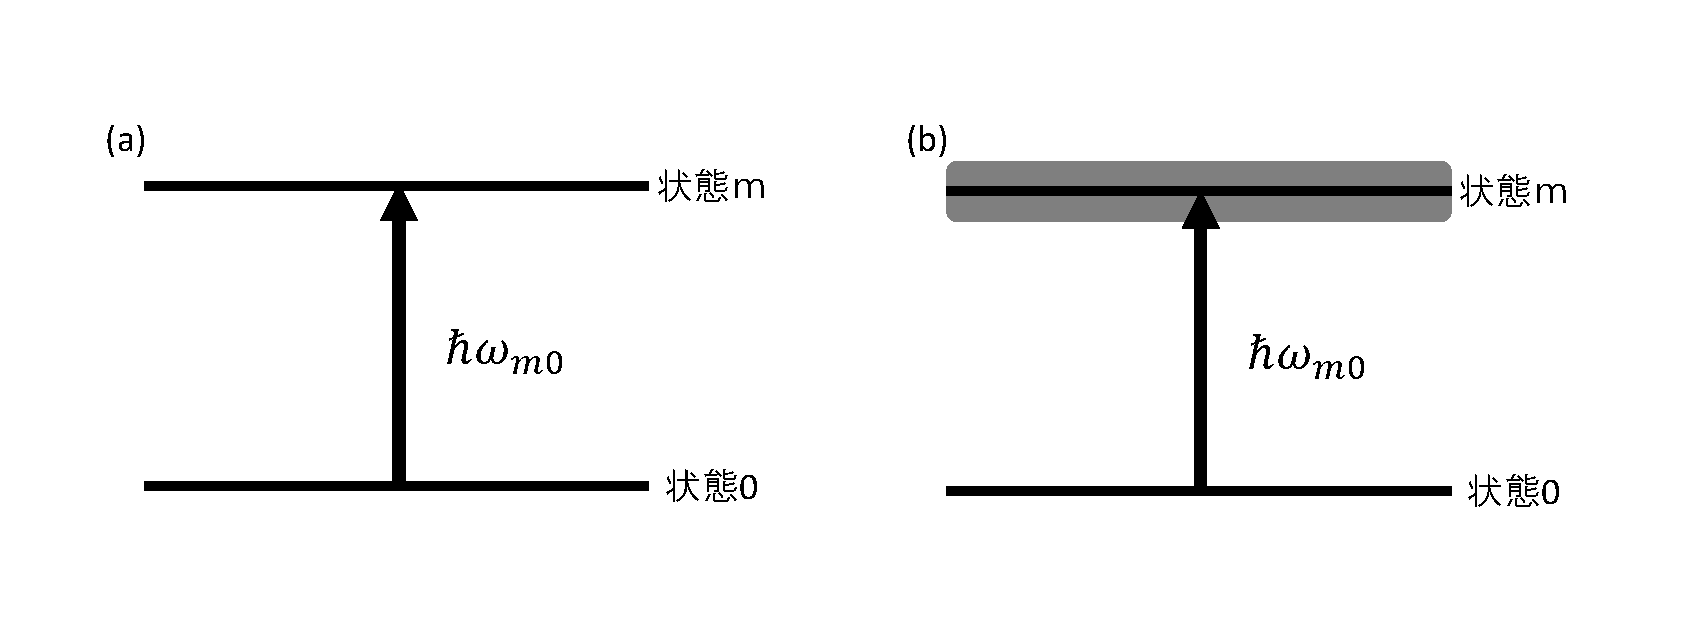
\includegraphics[width=12cm]{kadono2/img/seni.pdf}
      \caption{(a)離散的状態$m$への遷移、(b)連続的状態$m$への遷移}
      \label{fig:seni}
\end{figure}
(a)では数式(\ref{eq:risan})が利用でき、(b)では数式(\ref{eq:golden})が利用できる。\par


\section{複素積分}
数式(\ref{eq:hukuso})のところの積分は、めんどくさい積分。\par
変数変換とかしてとりあえず、
\begin{align}
    \int^\infty_0 \frac{\sin^2 x}{x^2}\mathrm{d}x = \frac{1}{2}\int^\infty_{-\infty} \frac{\sin^2 x}{x^2}\mathrm{d}x
\end{align}
という積分ということにする。被積分関数
\begin{align}
    f(z) = \frac{\sin^2z}{z^2}
\end{align}
は正則であるから、この関数を
\begin{align*}
    \oint f(z) \mathrm{d}z &= 0\\
    \oint = \int^{R-i}_{-R-i} + \int^{R}_{R-i} &+ \int^{-R}_{R} + \int^{-R-i}_{-R}
\end{align*}
という経路(図\ref{fig:sikaku})で積分して$R \to \infty$に飛ばしてやることを考える。\par
この経路にすることで、今後特異点をうまく避けることができる。
\begin{figure}[H]
    \centering
      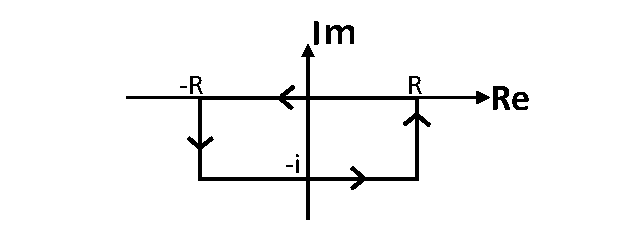
\includegraphics[height=2.5cm]{kadono2/img/hukuso1.pdf}
      \caption{$-i$下げる}
      \label{fig:sikaku}
\end{figure}
$R \to \infty$で上からおさえると$\int^{R}_{R-i} = \int^{-R-i}_{-R} = 0$となる!
\begin{align}
    -\int^{-R}_{R} &= \int^{R}_{-R}\frac{\sin^2x}{x^2}\mathrm{d}x
    = \int^{R-i}_{-R-i}\frac{\sin^2z}{z^2}\mathrm{d}z
    = \int^{R-i}_{-R-i} \frac{1-\cos(2z)}{2z^2}\mathrm{d}z \nonumber\\
    &= \int^{R-i}_{-R-i} \frac{1-\frac{e^{2iz}+e^{-2iz}}{2}}{2z^2} \mathrm{d}z
    = \int^{R-i}_{-R-i} \frac{2-e^{2iz}-e^{-2iz}}{4z^2} \mathrm{d}z\nonumber\\
    &= \int^{R-i}_{-R-i} \frac{1-e^{2iz}}{4z^2} \mathrm{d}z + \int^{R-i}_{-R-i} \frac{1-e^{-2iz}}{4z^2} \mathrm{d}z
    \label{eq:huku}
\end{align}
\begin{align}
    f_+(z) = \frac{1-e^{2iz}}{4z^2} && f_-(z) = \frac{1-e^{-2iz}}{4z^2}\nonumber
\end{align}
とおく。\par
経路に注意して複素積分してやると数式(\ref{eq:huku})を求めることができる。まず$f_+$を図の上を通る経路で
\begin{align}
    \oint f_+(z) \mathrm{d}z = \int^{R-i}_{-R-i} f_+(z) \mathrm{d}z + \int_{C_{上}} f_+(z) \mathrm{d}z
\end{align}
として、頑張ると$C_{上}$の経路はゼロになるはず、この経路の中には$z = 0$で特異点があるので、留数定理を使って
\begin{align}
    \int^{R-i}_{-R-i} f_+(z) \mathrm{d}z
    &= 2\pi i \Res_{z=0}[f_+] = 2\pi i \lim_{z \to 0}\frac{\mathrm{d}}{\mathrm{d}z}(z^2f_+) \nonumber\\
    &= 2\pi i \frac{1}{4}\lim_{z \to 0}\frac{\mathrm{d}}{\mathrm{d}z}(1-e^{2iz})\nonumber\\
    &= 2\pi i \frac{1}{4}\lim_{z \to 0}(-2ie^{2iz})\nonumber\\
    &= 2\pi i \times \frac{1}{4} \times (-2i) = \pi\nonumber
\end{align}
次に$f_-$を図の下を通る経路で
\begin{align*}
    \oint f_-(z) \mathrm{d}z = \int^{R-i}_{-R-i} f_-(z) \mathrm{d}z + \int_{C_{下}} f_-(z) \mathrm{d}z
\end{align*}
$C_{上}$の経路は頑張ればゼロにもっていける。この経路の中には特異点が存在しないので
\begin{align}
    \int^{R-i}_{-R-i} f_-(z) \mathrm{d}z = 0
\end{align}
したがって
\begin{align}
    \int^\infty_0 \frac{\sin^2 x}{x^2}\mathrm{d}x
    = \frac{1}{2}\int^\infty_{-\infty} \frac{\sin^2 x}{x^2}\mathrm{d}x
    = \frac{1}{2} \times \pi
    = \frac{\pi}{2}
\end{align}
\begin{figure}[H]
    \centering
    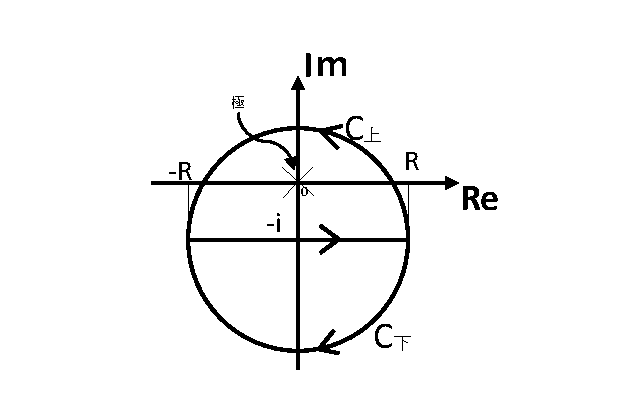
\includegraphics[height=3.5cm]{kadono2/img/hukuso2.pdf}
    \caption{数式\ref{eq:huku}を求める経路}
    \label{fig:maru}
\end{figure}
\vspace{-2zw}

% 参考文献
\sanko
\begin{enumerate}
\item 大成 誠之助著, 固体スペクトロスコピー, 裳華房, 1994.
\item 江藤 幹雄著, パリティ物理教科書シリーズ, 量子力学1, 丸善出版, 2013.
\item \url{http://www.nr.titech.ac.jp/~chiba/en/pdf/golden_rule_2.pdf}
\end{enumerate}


\end{document}
%
% ファイトだよ!
%